\documentclass[11pt,a4paper]{article}

% ============================================================
% VENI VIDI VICI - PARSEC
% Cybersecurity CTF
% Challenge Architecture & Technical Briefing
%
% Compile with:
%   pdflatex vvv_technical_briefing.tex
%   pdflatex vvv_technical_briefing.tex
% ============================================================


% ============================================================
% PACKAGES
% ============================================================

\usepackage[a4paper,margin=2.15cm]{geometry}

\usepackage[T1]{fontenc}
\usepackage[utf8]{inputenc}
\usepackage{lmodern}

\usepackage{amsmath}
\usepackage{amssymb}

\usepackage{xcolor}
\usepackage{graphicx}

\usepackage{booktabs}
\usepackage{tabularx}
\usepackage{array}
\usepackage{multirow}

\usepackage{enumitem}

\usepackage{tikz}
\usetikzlibrary{
    positioning,
    arrows.meta,
    shapes.geometric,
    fit,
    calc
}
\usetikzlibrary{positioning}

\usepackage{hyperref}
\usepackage{fancyhdr}
\usepackage{titlesec}
\usepackage{microtype}

% ============================================================
% COLORS
% ============================================================

\definecolor{VVVCyan}{RGB}{0,130,120}
\definecolor{VVVDark}{RGB}{35,35,35}
\definecolor{VVVGray}{RGB}{95,95,95}
\definecolor{VVVLight}{RGB}{242,244,245}
\definecolor{VVVLine}{RGB}{205,210,212}

% ============================================================
% HYPERREF
% ============================================================

\hypersetup{
    colorlinks=true,
    linkcolor=VVVCyan,
    urlcolor=VVVCyan,
    citecolor=VVVCyan,
    pdftitle={Veni Vidi Vici - Challenge Architecture and Technical Briefing},
    pdfauthor={Veni Vidi Vici Organizing Team}
}

% ============================================================
% GENERAL TYPOGRAPHY
% ============================================================

\setlength{\parindent}{0pt}
\setlength{\parskip}{6pt}

\setlist[itemize]{
    leftmargin=1.4em,
    itemsep=2pt,
    topsep=3pt
}

\setlist[enumerate]{
    leftmargin=1.6em,
    itemsep=3pt,
    topsep=3pt
}

\renewcommand{\arraystretch}{1.3}
\setlength{\tabcolsep}{5pt}

% ============================================================
% SECTION FORMATTING
% ============================================================

\titleformat{\section}
    {\Large\bfseries\color{VVVDark}}
    {\thesection}
    {0.7em}
    {}

\titleformat{\subsection}
    {\large\bfseries\color{VVVDark}}
    {\thesubsection}
    {0.6em}
    {}

\titleformat{\subsubsection}
    {\normalsize\bfseries\color{VVVCyan}}
    {\thesubsubsection}
    {0.5em}
    {}

\titlespacing*{\section}{0pt}{18pt}{8pt}
\titlespacing*{\subsection}{0pt}{12pt}{5pt}
\titlespacing*{\subsubsection}{0pt}{9pt}{4pt}

% ============================================================
% HEADER / FOOTER
% ============================================================

\pagestyle{fancy}

\fancyhf{}

\lhead{
    \small\textcolor{VVVGray}{Veni Vidi Vici}
}

\rhead{
    \small\textcolor{VVVGray}{PARSEC | IIT Dharwad}
}

\cfoot{
    \small\textcolor{VVVGray}{\thepage}
}

\renewcommand{\headrulewidth}{0.35pt}
\renewcommand{\footrulewidth}{0pt}

% ============================================================
% CUSTOM COMMANDS
% ============================================================

\newcommand{\domain}[1]{
    \vspace{0.3cm}
    {\large\bfseries\textcolor{VVVCyan}{#1}}
    \vspace{0.1cm}
}

\newcommand{\keypoint}[1]{
    \textbf{\textcolor{VVVDark}{#1}}
}

% ============================================================
% DOCUMENT
% ============================================================

\begin{document}

% ============================================================
% COVER PAGE
% ============================================================

\begin{titlepage}

\thispagestyle{empty}

\vspace*{1.2cm}

\begin{flushright}
    \textcolor{VVVGray}{\small PARSEC -- IIT Dharwad}
\end{flushright}

\vspace{2.0cm}

\begin{center}

{\Large
\textbf{\textcolor{VVVCyan}{VENI VIDI VICI}}
}

\vspace{0.3cm}

{\large
CYBERSECURITY CAPTURE THE FLAG
}

\vspace{1.5cm}

\rule{0.78\textwidth}{0.8pt}

\vspace{0.8cm}

{\Huge
\textbf{
Challenge Architecture\\
and Technical Briefing
}
}

\vspace{0.7cm}

{\Large
\textcolor{VVVGray}{
Proposed Structure for PARSEC
}
}

\vspace{1.5cm}

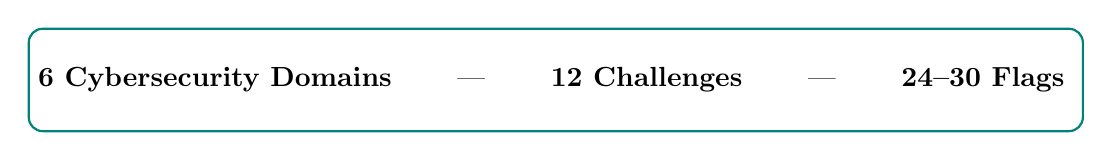
\begin{tikzpicture}

\node[
    draw=VVVCyan,
    line width=0.8pt,
    rounded corners=5pt,
    minimum width=11cm,
    minimum height=1.3cm,
    align=center
] {
    \textbf{6 Cybersecurity Domains}
    \hspace{0.6cm}
    |
    \hspace{0.6cm}
    \textbf{12 Challenges}
    \hspace{0.6cm}
    |
    \hspace{0.6cm}
    \textbf{24--30 Flags}
};

\end{tikzpicture}

\vspace{1.5cm}

{\large
\textit{
A practical, scenario-driven cybersecurity experience
}
}

\vfill

{\large
\textbf{Veni Vidi Vici Organizing Team}
}

\vspace{0.25cm}

{\large
PARSEC | IIT Dharwad
}

\vspace{0.8cm}

{\small
Technical Briefing | Proposed Architecture
}

\end{center}

\end{titlepage}


% ============================================================
% CONTENTS
% ============================================================

\tableofcontents

\newpage


% ============================================================
% 1. COMPETITION OVERVIEW
% ============================================================

\section{Competition Overview}

Veni Vidi Vici (VVV) is the proposed cybersecurity Capture The Flag
competition under PARSEC at IIT Dharwad.

The competition is intended to provide participants with a practical
security experience that goes beyond isolated puzzles and textbook
exercises.

The challenge set will be organized around six major cybersecurity
domains, with two primary challenge environments proposed for each
domain.

The current target is:

\begin{center}

\begin{tabular}{ccc}

\textbf{6} &
\textbf{12} &
\textbf{24--30}
\\

Domains &
Challenges &
Flags

\end{tabular}

\end{center}

The exact number of flags will remain flexible until the challenges
have been implemented and playtested.


\subsection{Competition Philosophy}

VVV is designed around the principle:

\begin{center}

\Large
\textbf{
Think like an attacker, reason like a defender.
}

\end{center}

Rather than simply asking participants to identify vulnerabilities,
the challenge environments should encourage them to:

\begin{itemize}

    \item investigate an unfamiliar system;

    \item identify its attack surface;

    \item understand how components interact;

    \item discover security weaknesses;

    \item exploit those weaknesses;

    \item progress through multiple stages where appropriate;

    \item and understand the security implications of their actions.

\end{itemize}


% ============================================================
% 2. ARCHITECTURE AT A GLANCE
% ============================================================

\section{Challenge Architecture at a Glance}

The challenge architecture is organized into three dimensions:

\begin{enumerate}

    \item \textbf{Domain} -- what area of cybersecurity the challenge
    focuses on.

    \item \textbf{Difficulty} -- the level of technical depth required.

    \item \textbf{Progression} -- how participants move from one
    objective to another within a challenge.

\end{enumerate}

\subsection{Six-Domain Architecture}

\begin{center}
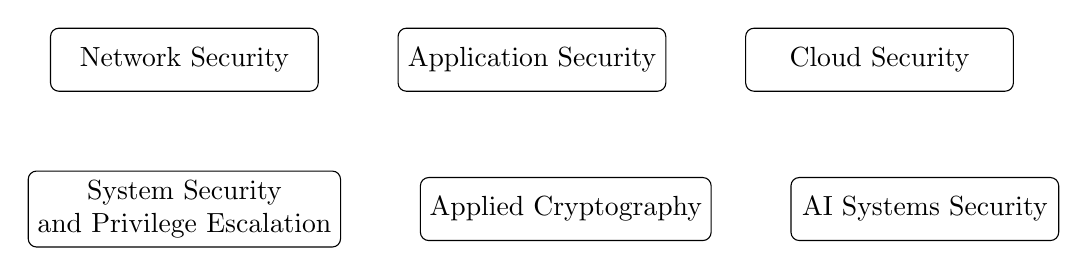
\begin{tikzpicture}[
    dbox/.style={
        rectangle,
        rounded corners=3pt,
        draw=black,
        minimum width=3.4cm,
        minimum height=0.8cm,
        align=center
    }
]

\node[dbox] (n)  {Network Security};
\node[dbox, right=of n]  (a)  {Application Security};
\node[dbox, right=of a]  (c)  {Cloud Security};

\node[dbox, below=of n]  (p)  {System Security\\and Privilege Escalation};
\node[dbox, right=of p]  (cr) {Applied Cryptography};
\node[dbox, right=of cr] (ai) {AI Systems Security};

\end{tikzpicture}
\end{center}


\subsection{Challenge Progression}

The challenge set is intended to move participants from foundational
tasks toward increasingly complex attack reasoning.

\begin{center}

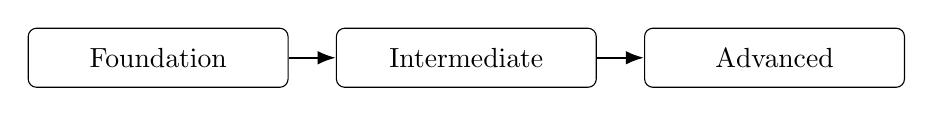
\begin{tikzpicture}[
    stage/.style={
        rectangle,
        rounded corners=3pt,
        draw=black,
        minimum width=3.3cm,
        minimum height=0.75cm,
        align=center
    }
]

\node[stage] (f)
{Foundation};

\node[stage, right=0.6cm of f] (i)
{Intermediate};

\node[stage, right=0.6cm of i] (a)
{Advanced};

\draw[-{Latex}, thick]
(f) -- (i);

\draw[-{Latex}, thick]
(i) -- (a);

\end{tikzpicture}

\end{center}

The progression is not intended to imply that every participant must
complete challenges sequentially. Participants should be able to
select challenges based on their skills and interests.


% ============================================================
% 3. CHALLENGE STRUCTURE
% ============================================================

\section{Challenge Structure}

The proposed structure consists of twelve primary challenge
environments.

Each challenge may contain multiple flags representing meaningful
milestones.

For example:

\begin{center}

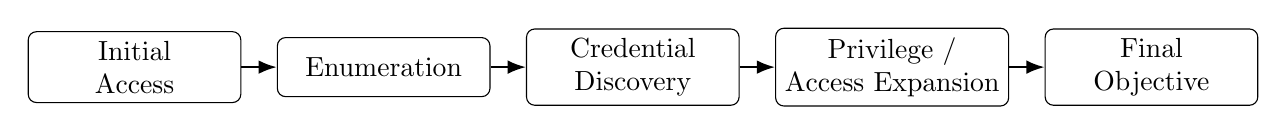
\begin{tikzpicture}[
    stage/.style={
        rectangle,
        rounded corners=3pt,
        draw=black,
        minimum width=2.7cm,
        minimum height=0.75cm,
        align=center
    }
]

\node[stage] (a)
{Initial\\Access};

\node[stage, right=0.45cm of a] (b)
{Enumeration};

\node[stage, right=0.45cm of b] (c)
{Credential\\Discovery};

\node[stage, right=0.45cm of c] (d)
{Privilege /\\Access Expansion};

\node[stage, right=0.45cm of d] (e)
{Final\\Objective};

\draw[-{Latex}, thick] (a) -- (b);
\draw[-{Latex}, thick] (b) -- (c);
\draw[-{Latex}, thick] (c) -- (d);
\draw[-{Latex}, thick] (d) -- (e);

\end{tikzpicture}

\end{center}

This means that a challenge can provide several meaningful points of
progress rather than having a single ``all-or-nothing'' flag.


% ============================================================
% 4. CHALLENGE MATRIX
% ============================================================

\section{Proposed Challenge Matrix}

The following matrix represents the current architectural baseline.

\begin{center}

\small

\begin{tabularx}{\textwidth}{
    >{\bfseries}p{0.7cm}
    >{\bfseries}p{3.1cm}
    p{2.4cm}
    >{\centering\arraybackslash}p{1.1cm}
    X
}

\toprule

ID &
Domain &
Difficulty &
Flags &
Primary Concepts \\

\midrule

N1 &
Network Security &
Foundation &
2 &
Reconnaissance, service enumeration \\

N2 &
Network Security &
Intermediate &
3 &
Traffic analysis, internal discovery, pivoting \\

A1 &
Application Security &
Foundation &
2 &
Web and API security fundamentals \\

A2 &
Application Security &
Intermediate / Advanced &
4 &
Multi-stage application exploitation \\

C1 &
Cloud Security &
Foundation / Intermediate &
2 &
IAM, configuration and access control \\

C2 &
Cloud Security &
Advanced &
3 &
Cloud privilege and attack paths \\

P1 &
System Security &
Intermediate &
2 &
Local privilege escalation \\

P2 &
System Security &
Advanced &
4 &
Compromised host and multi-stage escalation \\

CR1 &
Applied Cryptography &
Foundation / Intermediate &
1--2 &
Cryptographic misuse \\

CR2 &
Applied Cryptography &
Advanced &
2 &
Protocol or mathematical weakness \\

AI1 &
AI Systems Security &
Intermediate &
2 &
RAG and AI application security \\

AI2 &
AI Systems Security &
Advanced &
3--4 &
AI agents and tool security \\

\bottomrule

\end{tabularx}

\end{center}


\subsection{Target Distribution}

The intended distribution is approximately:

\begin{center}

\begin{tabular}{lcc}

\toprule

\textbf{Difficulty} &
\textbf{Challenges} &
\textbf{Purpose}
\\

\midrule

Foundation &
4 &
Accessibility and onboarding
\\

Intermediate &
5 &
Core technical depth
\\

Advanced &
3 &
High-complexity attack chains
\\

\bottomrule

\end{tabular}

\end{center}

This distribution is provisional and may be adjusted after
playtesting.


% ============================================================
% 5. DOMAIN I
% ============================================================

\section{Domain I -- Network Security}

Network Security focuses on networks, exposed services, protocols,
traffic, and internal infrastructure.

\subsection{Primary Concepts}

\begin{itemize}

    \item Reconnaissance and enumeration
    \item Port and service discovery
    \item Service fingerprinting
    \item Network mapping
    \item Packet and PCAP analysis
    \item Protocol analysis
    \item Insecure protocols
    \item Authentication weaknesses
    \item Network segmentation
    \item Internal service discovery
    \item Pivoting and lateral movement

\end{itemize}


\subsection{N1 -- Network Reconnaissance}

The introductory challenge is intended to establish the fundamental
workflow of identifying and understanding an exposed attack surface.

Participants may be required to identify services, understand their
behavior, and locate an initial security weakness.


\subsection{N2 -- Internal Network}

The intermediate environment introduces the concept that obtaining
access to one system does not necessarily represent the end of an
attack.

A conceptual progression is:

\[
\text{External Service}
\rightarrow
\text{Initial Access}
\rightarrow
\text{Internal Enumeration}
\rightarrow
\text{Pivot}
\rightarrow
\text{Internal Objective}
\]


% ============================================================
% 6. DOMAIN II
% ============================================================

\section{Domain II -- Application Security}

Application Security focuses on web applications, APIs,
authentication, authorization, and application-level trust
boundaries.


\subsection{Primary Concepts}

\begin{itemize}

    \item Injection vulnerabilities
    \item Cross-site scripting
    \item Path traversal
    \item Server-side request forgery
    \item Command injection
    \item Broken access control
    \item IDOR / BOLA
    \item Authentication bypass
    \item Session and JWT security
    \item File upload vulnerabilities
    \item Business-logic vulnerabilities

\end{itemize}


\subsection{A1 -- Web and API Security}

The foundation application challenge introduces participants to
application reconnaissance and common security boundaries.


\subsection{A2 -- Multi-Stage Application Attack}

The advanced application environment may combine multiple weaknesses
into a single scenario:

\[
\text{Application Exposure}
\rightarrow
\text{Initial Access}
\rightarrow
\text{Credential Discovery}
\rightarrow
\text{Internal Resource}
\rightarrow
\text{Final Objective}
\]


% ============================================================
% 7. DOMAIN III
% ============================================================

\section{Domain III -- Cloud Security}

Cloud Security introduces identity, access control, resource
configuration, and service relationships.


\subsection{Primary Concepts}

\begin{itemize}

    \item Identity and Access Management
    \item Least privilege
    \item Excessive permissions
    \item Cloud storage security
    \item Publicly exposed resources
    \item Credential and secret leakage
    \item Service-to-service trust
    \item Metadata access
    \item Cloud privilege escalation
    \item Cloud attack paths

\end{itemize}


\subsection{C1 -- Cloud Configuration}

The introductory environment focuses on identifying insecure
configuration and excessive permissions.


\subsection{C2 -- Cloud Attack Path}

The advanced challenge may combine an application or service
compromise with cloud identity and access-control weaknesses.

Cloud environments will be isolated or simulated and will not expose
production infrastructure.


% ============================================================
% 8. DOMAIN IV
% ============================================================

\section{Domain IV -- System Security and Privilege Escalation}

This domain focuses on operating-system security and privilege
boundaries.

\subsection{Linux Concepts}

\begin{itemize}

    \item File permissions
    \item SUID and SGID
    \item Linux capabilities
    \item Sudo configuration
    \item Cron jobs
    \item Services
    \item Environment variables
    \item Writable files and directories

\end{itemize}


\subsection{Windows Concepts}

\begin{itemize}

    \item Services
    \item Scheduled tasks
    \item Permissions
    \item Credential discovery
    \item Privilege boundaries

\end{itemize}


\subsection{P1 -- Local Privilege Escalation}

Participants begin with restricted access and must enumerate the
environment before identifying a privilege-boundary weakness.


\subsection{P2 -- Compromised Host}

The advanced challenge may combine:

\[
\text{Initial Foothold}
\rightarrow
\text{Enumeration}
\rightarrow
\text{Credential Discovery}
\rightarrow
\text{Lateral Movement}
\rightarrow
\text{Privilege Escalation}
\rightarrow
\text{Objective}
\]


% ============================================================
% 9. DOMAIN V
% ============================================================

\section{Domain V -- Applied Cryptography}

Applied Cryptography focuses on practical weaknesses in cryptographic
systems rather than simple ciphertext decoding.


\subsection{Primary Concepts}

\begin{itemize}

    \item Cryptanalysis
    \item Symmetric cryptographic misuse
    \item IV and nonce misuse
    \item Weak randomness
    \item RSA weaknesses
    \item Key management
    \item Digital signature failures
    \item Cryptographic protocols
    \item Implementation weaknesses
    \item Mathematical reasoning

\end{itemize}


\subsection{CR1 -- Cryptographic Misuse}

A practical problem involving an incorrectly implemented or incorrectly
used cryptographic construction.


\subsection{CR2 -- Advanced Cryptographic Security}

A more demanding challenge involving protocol analysis, mathematical
reasoning, or implementation-level weaknesses.


% ============================================================
% 10. DOMAIN VI
% ============================================================

\section{Domain VI -- AI Systems Security}

AI Systems Security is included as a dedicated domain covering
security issues in modern AI-enabled applications and systems.


\subsection{Primary Concepts}

\begin{itemize}

    \item Prompt and instruction security
    \item Direct and indirect prompt injection
    \item Context manipulation
    \item Retrieval-Augmented Generation security
    \item Retrieval poisoning
    \item Vector-store access control
    \item AI agent security
    \item Tool and API abuse
    \item Excessive agent permissions
    \item AI application security
    \item Model security
    \item AI supply-chain security

\end{itemize}


\subsection{AI1 -- RAG and AI Application Security}

The intermediate environment focuses on the trust boundaries between
an AI model, its context, retrieval system, and protected data.


\subsection{AI2 -- AI Agent Security}

The advanced environment may explore the consequences of connecting
an AI agent to tools, APIs, files, or backend services.

A conceptual architecture is:

\[
\text{LLM}
\rightarrow
\text{Agent}
\rightarrow
\text{Tools}
\rightarrow
\text{Backend Services}
\rightarrow
\text{Protected Resource}
\]

AI challenges should use controlled and sandboxed environments so
that model behavior does not make challenge outcomes unpredictable.


% ============================================================
% 11. REAL-WORLD SCENARIO DESIGN
% ============================================================

\section{Real-World Scenario Design}

A central objective of VVV is to move away from purely puzzle-oriented
challenges toward scenario-driven security problems.

Instead of presenting a participant with only:

\begin{center}
\textit{``Find the flag.''}
\end{center}

the challenge should provide a context in which the participant must
understand a system and determine how it can be compromised.

For example, a challenge may present:

\begin{center}

\textit{
A company has deployed an internal API. An authorization boundary
has been incorrectly implemented. Investigate the application,
identify the security weakness, and obtain access to the protected
resource.
}

\end{center}

The exact scenario will vary by challenge, but the general principle
is that participants should be solving a security problem rather than
simply locating an arbitrary string.


% ============================================================
% 12. CROSS-DOMAIN CHALLENGES
% ============================================================

\section{Cross-Domain Attack Chains}

Selected advanced challenges may intentionally combine multiple
domains.

A representative attack chain may look like:

\begin{center}

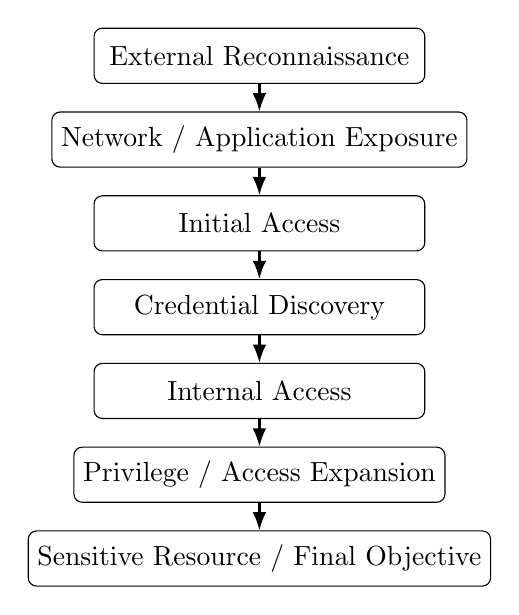
\begin{tikzpicture}[
    stage/.style={
        rectangle,
        rounded corners=3pt,
        draw=black,
        minimum width=4.2cm,
        minimum height=0.7cm,
        align=center
    }
]

\node[stage] (r)
{External Reconnaissance};

\node[stage, below=0.35cm of r] (a)
{Network / Application Exposure};

\node[stage, below=0.35cm of a] (i)
{Initial Access};

\node[stage, below=0.35cm of i] (c)
{Credential Discovery};

\node[stage, below=0.35cm of c] (l)
{Internal Access};

\node[stage, below=0.35cm of l] (p)
{Privilege / Access Expansion};

\node[stage, below=0.35cm of p] (o)
{Sensitive Resource / Final Objective};

\draw[-{Latex}, thick] (r) -- (a);
\draw[-{Latex}, thick] (a) -- (i);
\draw[-{Latex}, thick] (i) -- (c);
\draw[-{Latex}, thick] (c) -- (l);
\draw[-{Latex}, thick] (l) -- (p);
\draw[-{Latex}, thick] (p) -- (o);

\end{tikzpicture}

\end{center}

The purpose is to expose participants to the idea that real-world
security incidents often involve multiple interacting weaknesses.


% ============================================================
% 13. TECHNICAL INFRASTRUCTURE
% ============================================================

\section{Technical Infrastructure}

The implementation architecture will prioritize isolation,
repeatability, and maintainability.

The conceptual participant flow is:

\begin{center}

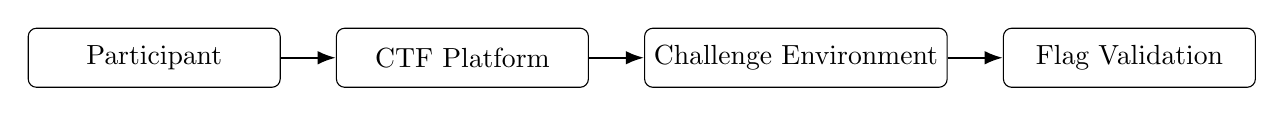
\begin{tikzpicture}[
    stage/.style={
        rectangle,
        rounded corners=3pt,
        draw=black,
        minimum width=3.2cm,
        minimum height=0.75cm,
        align=center
    }
]

\node[stage] (p)
{Participant};

\node[stage, right=0.7cm of p] (c)
{CTF Platform};

\node[stage, right=0.7cm of c] (e)
{Challenge Environment};

\node[stage, right=0.7cm of e] (f)
{Flag Validation};

\draw[-{Latex}, thick] (p) -- (c);
\draw[-{Latex}, thick] (c) -- (e);
\draw[-{Latex}, thick] (e) -- (f);

\end{tikzpicture}

\end{center}


\subsection{Infrastructure Principles}

The challenge infrastructure should support:

\begin{itemize}

    \item isolated environments,

    \item reproducible deployment,

    \item automated reset,

    \item deterministic flag validation,

    \item reusable base environments,

    \item controlled resource consumption,

    \item monitoring and troubleshooting.

\end{itemize}


\subsection{Isolation and Safety}

All intentionally vulnerable systems should be isolated from
production infrastructure.

Participants should never receive access to:

\begin{itemize}

    \item real organizational credentials,

    \item production cloud accounts,

    \item production databases,

    \item unrestricted external systems.

\end{itemize}

The competition infrastructure should be designed so that
participants can safely experiment within the intended challenge
boundaries.


% ============================================================
% 14. CHALLENGE DEVELOPMENT
% ============================================================

\section{Challenge Development and Testing}

Every challenge should pass through a defined development cycle.

\begin{center}

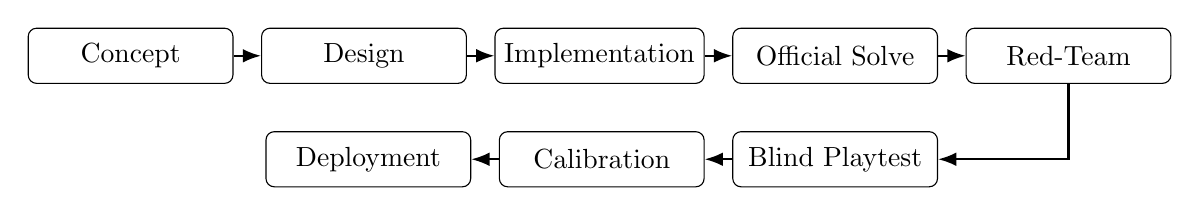
\begin{tikzpicture}[
    stage/.style={
        rectangle,
        rounded corners=3pt,
        draw=black,
        minimum width=2.6cm,
        minimum height=0.7cm,
        align=center
    }
]

\node[stage] (a)
{Concept};

\node[stage, right=0.35cm of a] (b)
{Design};

\node[stage, right=0.35cm of b] (c)
{Implementation};

\node[stage, right=0.35cm of c] (d)
{Official Solve};

\node[stage, right=0.35cm of d] (e)
{Red-Team};

\node[stage, below=0.6cm of d] (f)
{Blind Playtest};

\node[stage, left=0.35cm of f] (g)
{Calibration};

\node[stage, left=0.35cm of g] (h)
{Deployment};

\draw[-{Latex}, thick] (a) -- (b);
\draw[-{Latex}, thick] (b) -- (c);
\draw[-{Latex}, thick] (c) -- (d);
\draw[-{Latex}, thick] (d) -- (e);

\draw[-{Latex}, thick] (e) |- (f);
\draw[-{Latex}, thick] (f) -- (g);
\draw[-{Latex}, thick] (g) -- (h);

\end{tikzpicture}

\end{center}


\subsection{Testing Requirements}

Before deployment, each challenge should undergo:

\begin{enumerate}

    \item Intended-solution validation.
    \item Deployment and reset testing.
    \item Unintended-solution testing.
    \item Resource and stability testing.
    \item Blind playtesting.
    \item Difficulty calibration.

\end{enumerate}


% ============================================================
% 15. INDUSTRY AND SPONSOR INTEGRATION
% ============================================================

\section{Industry and Sponsor Integration}

Industry participation can significantly improve the realism and
relevance of VVV challenges.

Sponsors may contribute:

\begin{itemize}

    \item industry-inspired security scenarios,

    \item application security problems,

    \item cloud security scenarios,

    \item network security scenarios,

    \item incident-response scenarios,

    \item cryptographic problems,

    \item AI security scenarios,

    \item multi-stage attack scenarios.

\end{itemize}


\subsection{Sponsor Problem Statement Model}

A sponsor does not necessarily need to provide a complete CTF
challenge.

A problem statement, security scenario, vulnerability class, or
industry-inspired case can be adapted by the VVV organizing team.

\begin{center}


\begin{tikzpicture}[
    stage/.style={
        rectangle,
        rounded corners=3pt,
        draw=black,
        minimum width=3.1cm,
        minimum height=0.75cm,
        align=center
    }
]

\node[stage] (s)
{Industry Scenario};

\node[stage, right=0.5cm of s] (v)
{VVV Technical\\Adaptation};

\node[stage, right=0.5cm of v] (b)
{Sandbox and\\Safety Review};

\node[stage, right=0.5cm of b] (c)
{Competition\\Challenge};

\draw[-{Latex}, thick] (s) -- (v);
\draw[-{Latex}, thick] (v) -- (b);
\draw[-{Latex}, thick] (b) -- (c);

\end{tikzpicture}

\end{center}

This model allows industry partners to contribute technical expertise
without requiring them to build and operate the entire competition
infrastructure.


% ============================================================
% 16. EXPECTED PARTICIPANT EXPERIENCE
% ============================================================

\section{Expected Participant Experience}

The intended experience can be summarized as:

\begin{center}

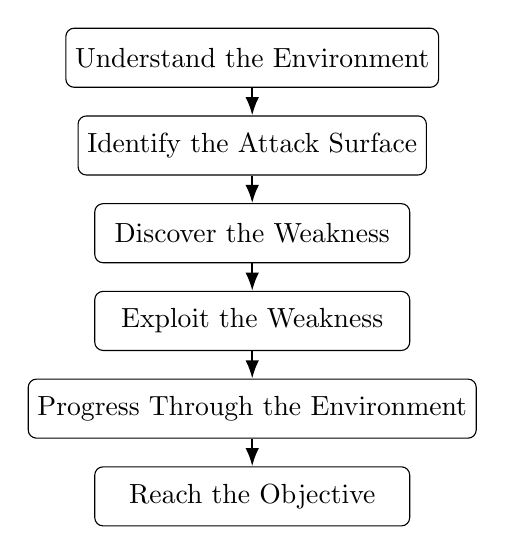
\begin{tikzpicture}[
    stage/.style={
        rectangle,
        rounded corners=3pt,
        draw=black,
        minimum width=4cm,
        minimum height=0.75cm,
        align=center
    }
]

\node[stage] (a)
{Understand the Environment};

\node[stage, below=0.35cm of a] (b)
{Identify the Attack Surface};

\node[stage, below=0.35cm of b] (c)
{Discover the Weakness};

\node[stage, below=0.35cm of c] (d)
{Exploit the Weakness};

\node[stage, below=0.35cm of d] (e)
{Progress Through the Environment};

\node[stage, below=0.35cm of e] (f)
{Reach the Objective};

\draw[-{Latex}, thick] (a) -- (b);
\draw[-{Latex}, thick] (b) -- (c);
\draw[-{Latex}, thick] (c) -- (d);
\draw[-{Latex}, thick] (d) -- (e);
\draw[-{Latex}, thick] (e) -- (f);

\end{tikzpicture}

\end{center}

The desired outcome is for participants to leave with experience in
security investigation and reasoning rather than only a collection of
individual exploitation techniques.


% ============================================================
% 17. SCOPE
% ============================================================

\section{Scope and Design Boundaries}

The current scope is intentionally limited to twelve primary
challenge environments.

The competition will prioritize:

\begin{itemize}

    \item technical depth,

    \item realistic scenarios,

    \item reliable infrastructure,

    \item progressive difficulty,

    \item meaningful flags,

    \item cross-domain reasoning,

    \item safe sandboxed execution.

\end{itemize}

The architecture does not require every challenge to use complex
infrastructure.

Instead, infrastructure complexity will be introduced only where it
meaningfully contributes to the intended security experience.


% ============================================================
% 18. SUMMARY
% ============================================================

\section{Architecture Summary}

\begin{center}

\begin{tabular}{ll}

\toprule

\textbf{Component} & \textbf{Proposed Structure} \\

\midrule

Cybersecurity Domains &
6 \\

Primary Challenges &
12 \\

Target Flags &
24--30 \\

Difficulty Levels &
Foundation, Intermediate, Advanced \\

Challenge Style &
Scenario-driven and hands-on \\

Advanced Design &
Multi-stage and cross-domain attack chains \\

Cloud Environment &
Sandboxed / simulated \\

AI Environment &
Controlled and sandboxed \\

Infrastructure &
Isolated and reproducible \\

Testing &
Internal, red-team, and blind playtesting \\

Industry Integration &
Sponsor-provided scenarios and problem statements \\

\bottomrule

\end{tabular}

\end{center}


% ============================================================
% CONCLUSION
% ============================================================

\newpage

\section*{Conclusion}

\addcontentsline{toc}{section}{Conclusion}

Veni Vidi Vici is envisioned as a practical cybersecurity competition
that combines six areas of modern security into a coherent
participant experience.

The proposed structure of twelve challenges and approximately
24--30 flags is intended to balance technical depth with the
practical constraints of challenge development and infrastructure
management.

The central design principle is simple:

\begin{center}

\Large
\textbf{
Do not just find the vulnerability.
Understand the system, exploit the weakness, and reason about the
attack.
}

\end{center}

The architecture is intentionally flexible so that relevant
industry-generated problem statements can be incorporated during
challenge development.

\vfill

\begin{center}

\textbf{VENI VIDI VICI}

\vspace{0.15cm}

Cybersecurity Capture The Flag

\vspace{0.15cm}

PARSEC | IIT Dharwad

\end{center}


% ============================================================
% END
% ============================================================

\end{document}